\EnglishSourceFrame{GELFAND-P001465}{65}
The product $BA$ is represented by joining:

(18) \EnglishSourceFigure{GELFAND-P001465}{eq18-composition}{On the left is a rectangle labelled $BA$, with three strands above and three below. Above the upper ends are $m'_1,m'_2,m'_M$; beside the upper strands, $j'_1,j'_2,j'_M$; beside the lower strands, $j_1,j_2,j_L$, and below, $m_1,m_2,m_L$. After an equals sign are two rectangles, $B$ above $A$, joined by three strands. Beside the upper strands of $B$ are $j''_1,j''_2$ and $j_M$ with an uncertain prime; above the right-hand strand is $m'_M$. The first two upper ends approach the heading line. On the connecting strands are $j'_1,j'_2,j'_L$. Beside the lower strands of $A$ are $j_1,j_2$ and a sign resembling $j_M$; below are $m_1,m_2,m_L$. Next is an equals sign, a sum labelled $m'_1\ldots m'_L$, and two separate rectangles, unlabelled inside, one above the other. Each has three ends above and below; between the rectangles are $m'_1,m'_2,m'_L$. The number of primes on some $j$ labels and the final lower index beside $A$ require comparison with the original.}

\par\medskip\noindent
\begin{minipage}[c]{0.48\linewidth}\centering
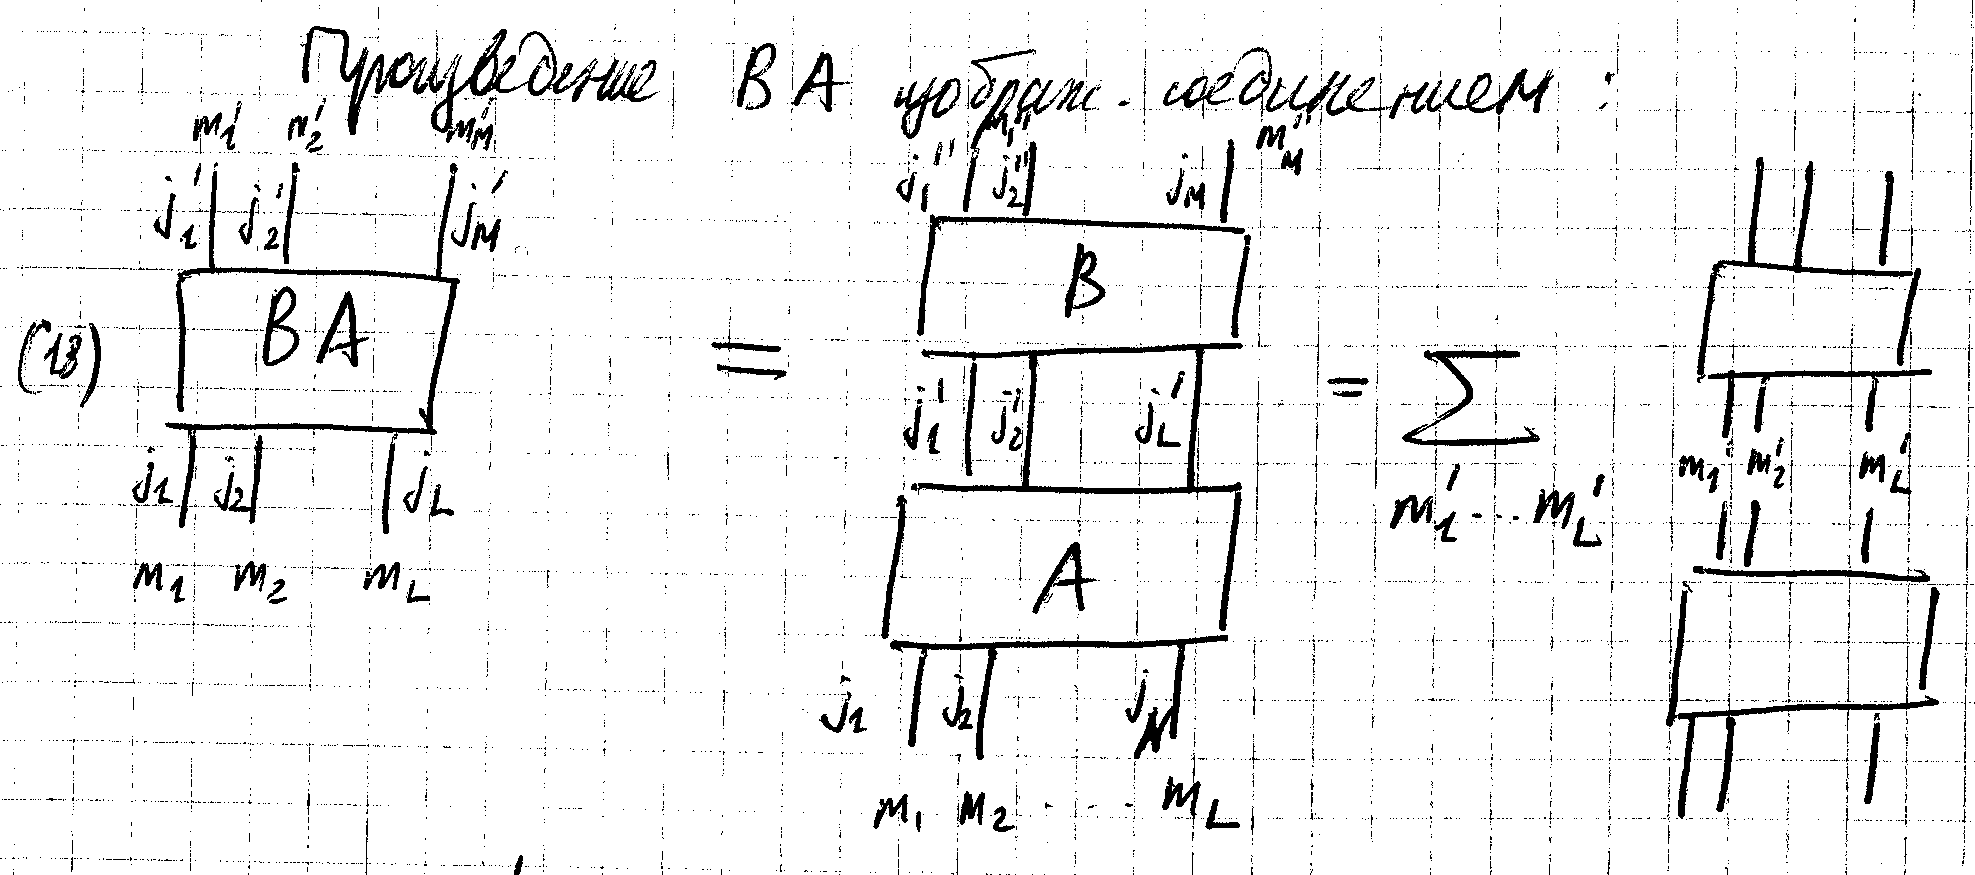
\includegraphics[width=\linewidth]{figures/gelfand-p001465-eq18-composition-original.png}
\par\smallskip{\footnotesize Original manuscript diagram: GELFAND-P001465\par}
\end{minipage}\hfill
\begin{minipage}[c]{0.48\linewidth}\centering
\resizebox{\linewidth}{!}{% Partial recreation. All uncertain indices/primes are explicitly bracketed.
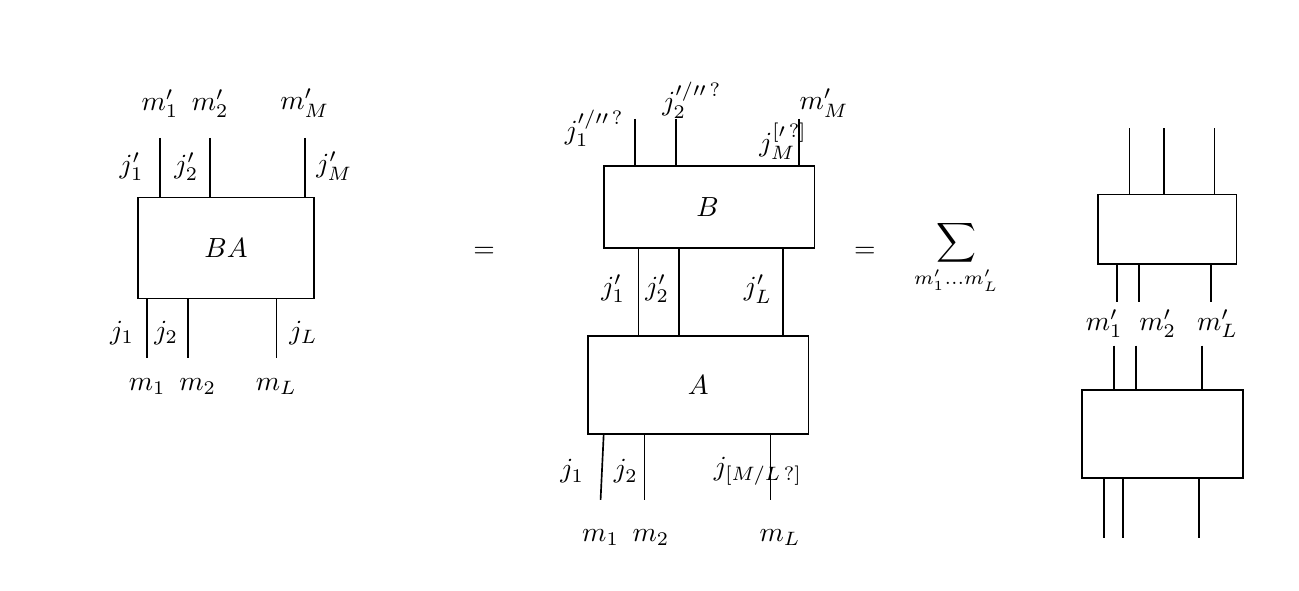
\begin{tikzpicture}[x=0.008cm,y=-0.008cm,line width=0.6pt]
\path[use as bounding box] (0,0) rectangle (1975,850);
\draw (175,270) rectangle (455,430);
\node at (315,350) {$BA$};
\foreach \x in {210,290,440}{\draw (\x,175)--(\x,270);}
\foreach \x in {190,255,395}{\draw (\x,430)--(\x,525);}
\node at (210,120) {$m'_1$};\node at (290,120) {$m'_2$};\node at (440,120) {$m'_M$};
\node at (165,220) {$j'_1$};\node at (252,220) {$j'_2$};\node at (487,220) {$j'_M$};
\node at (150,485) {$j_1$};\node at (220,485) {$j_2$};\node at (438,485) {$j_L$};
\node at (190,570) {$m_1$};\node at (270,570) {$m_2$};\node at (395,570) {$m_L$};
\node at (725,357) {$=$};
\draw (915,220) rectangle (1250,350);\node at (1080,285) {$B$};
\draw (890,490) rectangle (1240,645);\node at (1065,567) {$A$};
\foreach \x in {965,1030,1225}{\draw (\x,145)--(\x,220);}
\draw (970,350)--(970,490);\draw (1035,350)--(1035,490);\draw (1200,350)--(1200,490);
\draw (915,645)--(910,750);\draw (980,645)--(980,750);\draw (1180,645)--(1180,750);
\node at (900,160) {$j_1^{\prime/\prime\prime\,?}$};
\node at (1055,115) {$j_2^{\prime/\prime\prime\,?}$};
\node at (1200,180) {$j_M^{[\prime\,?]}$};\node at (1265,120) {$m'_M$};
\node at (930,415) {$j'_1$};\node at (1000,415) {$j'_2$};\node at (1160,415) {$j'_L$};
\node at (865,705) {$j_1$};\node at (950,705) {$j_2$};\node at (1160,705) {$j_{[M/L\,?]}$};
\node at (910,810) {$m_1$};\node at (990,810) {$m_2$};\node at (1195,810) {$m_L$};
\node at (1330,357) {$=$};\node at (1475,365) {$\displaystyle\sum_{m'_1\ldots m'_L}$};
\draw (1700,265) rectangle (1920,375);\draw (1675,575) rectangle (1930,715);
\foreach \x in {1750,1805,1885}{\draw (\x,160)--(\x,265);}
\foreach \x in {1730,1765,1880}{\draw (\x,375)--(\x,435);}
\foreach \x in {1725,1760,1865}{\draw (\x,505)--(\x,575);}
\foreach \x in {1710,1740,1860}{\draw (\x,715)--(\x,810);}
\node at (1710,470) {$m'_1$};\node at (1795,470) {$m'_2$};\node at (1890,470) {$m'_L$};
\end{tikzpicture}
}
\par\smallskip{\footnotesize Partial recreation of visible strokes; uncertain labels and connections remain explicit.\par}
\end{minipage}\par\medskip


\begin{equation*}
V^j\overset{id}{\longrightarrow}V^j
\quad\text{represented by a strand}\quad
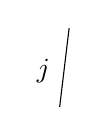
\begin{tikzpicture}[baseline=(current bounding box.center),x=1cm,y=1cm]
\draw (0,0)--(0.12,1);
\node[left] at (0,0.45) {$j$};
\end{tikzpicture}
\tag{19}
\end{equation*}

(20) \EnglishSourceFigure{GELFAND-P001465}{eq20-crossing}{Two crossing strands. Upper left: $j_2$; upper right: $j_1$; lower left: $j_1$; lower right: $j_2$. The strand from upper left to lower right is continuous; the other is interrupted at the crossing. At the lower-right end is a thickened pointed stroke; its arrow direction is not established.}

\par\medskip\noindent
\begin{minipage}[c]{0.48\linewidth}\centering
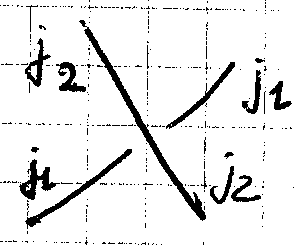
\includegraphics[width=\linewidth]{figures/gelfand-p001465-eq20-crossing-original.png}
\par\smallskip{\footnotesize Original manuscript diagram: GELFAND-P001465\par}
\end{minipage}\hfill
\begin{minipage}[c]{0.48\linewidth}\centering
\resizebox{\linewidth}{!}{% The single side hook is traced; no arrow direction is asserted.
\begin{tikzpicture}[x=0.015cm,y=-0.015cm,line width=0.7pt]
\path[use as bounding box] (0,0) rectangle (295,245);
\draw (85,25)--(205,215);\draw (205,215)--(205,201);
\draw (29,220)--(125,152);\draw (168,126)..controls(205,101)and(218,77)..(232,64);
\node at (50,65) {$j_2$};\node at (264,94) {$j_1$};
\node at (44,177) {$j_1$};\node at (253,185) {$j_2$};
\end{tikzpicture}
}
\par\smallskip{\footnotesize Partial recreation of visible strokes; uncertain labels and connections remain explicit.\par}
\end{minipage}\par\medskip

\EnglishUnclear{GELFAND-P001465}{eq20-v-indices}{$R^{j_1j_2}:V^{j_1}\otimes V^{j_1}\longrightarrow V^{j_1}\otimes V^{j_1}$}

\begin{equation*}
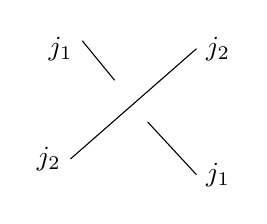
\begin{tikzpicture}[baseline=(current bounding box.center),x=1cm,y=1cm]
\draw (-0.8,-0.7)--(0.8,0.7);
\draw (-0.65,0.8)--(-0.24,0.30);
\draw (0.18,-0.23)--(0.8,-0.9);
\node[left] at (-0.65,0.7) {$j_1$};
\node[right] at (0.8,0.7) {$j_2$};
\node[left] at (-0.8,-0.7) {$j_2$};
\node[right] at (0.8,-0.9) {$j_1$};
\end{tikzpicture}
\qquad (R^{j_2j_1})^{-1}\qquad\text{in the same space}
\tag{20'}
\end{equation*}

\begin{equation*}
RR^{-1}=I\qquad
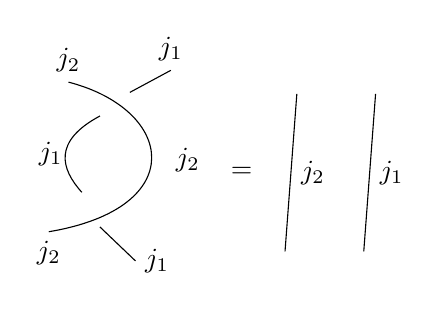
\begin{tikzpicture}[baseline=(current bounding box.center),x=1cm,y=1cm]
\draw (-0.55,1.15).. controls (0.8,0.8) and (1.0,-0.45)..(-0.8,-0.75);
\draw (0.75,1.3)--(0.23,1.02);
\draw (-0.15,0.72).. controls (-0.75,0.4) and (-0.65,0.05)..(-0.38,-0.25);
\draw (-0.15,-0.69)--(0.30,-1.12);
\node[above] at (-0.55,1.15) {$j_2$};
\node[above] at (0.75,1.3) {$j_1$};
\node[left] at (-0.50,0.24) {$j_1$};
\node[right] at (0.69,0.16) {$j_2$};
\node[below] at (-0.8,-0.75) {$j_2$};
\node[right] at (0.30,-1.12) {$j_1$};
\node at (1.65,0) {$=$};
\draw (2.2,-1)--(2.35,1);
\draw (3.2,-1)--(3.35,1);
\node[right] at (2.28,0) {$j_2$};
\node[right] at (3.28,0) {$j_1$};
\end{tikzpicture}
\end{equation*}

$j_1,j_2$ are the colours of the strands.

[The source heading has a wavy underline.]
\underline{The Yang--Baxter relation}

\begin{equation*}
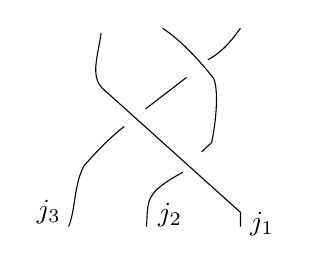
\begin{tikzpicture}[baseline=(current bounding box.center),x=0.006cm,y=-0.006cm]
\draw (70,10).. controls (62,65) and (45,106)..(78,132)
 --(365,390)--(365,420);
\draw (200,0).. controls (243,28) and (286,78)..(308,106)
 .. controls (319,130) and (314,195)..(304,242)--(283,262);
\draw (243,305).. controls (160,350) and (170,365)..(166,420);
\draw (1,420).. controls (16,385) and (12,330)..(34,291)
 .. controls (64,257) and (86,234)..(119,208);
\draw (164,171)--(251,104);
\draw (296,67).. controls (333,46) and (350,20)..(365,0);
\node[left] at (5,389) {$j_3$};
\node[right] at (170,396) {$j_2$};
\node[right] at (365,414) {$j_1$};
\end{tikzpicture}
\quad =\quad
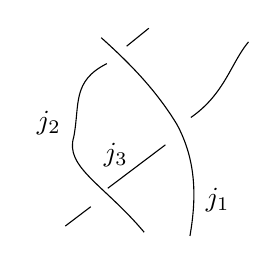
\begin{tikzpicture}[baseline=(current bounding box.center),x=0.006cm,y=-0.006cm]
\draw (90,20).. controls (164,86) and (212,141)..(250,203)
 .. controls (292,280) and (292,360)..(278,440);
\draw (191,0)--(144,38);
\draw (102,75).. controls (28,112) and (45,161)..(32,230)
 .. controls (12,294) and (96,331)..(181,432);
\draw (14,419)--(68,378);
\draw (104,339)--(226,247);
\draw (280,189).. controls (352,139) and (365,73)..(402,29);
\node[left] at (25,200) {$j_2$};
\node at (121,268) {$j_3$};
\node[right] at (291,364) {$j_1$};
\end{tikzpicture}
\tag{21}
\end{equation*}

Additional vertices

\begin{equation*}
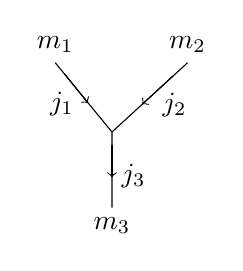
\begin{tikzpicture}[baseline=(current bounding box.center),x=0.8cm,y=0.8cm]
\draw (-0.9,1.1)--(0,0)--(0,-1.2);
\draw (1.2,1.1)--(0,0);
\draw[->] (-0.75,0.92)--(-0.38,0.46);
\draw[->] (0.97,0.89)--(0.48,0.44);
\draw[->] (0,-0.2)--(0,-0.72);
\node[above] at (-0.9,1.1) {$m_1$};
\node[above] at (1.2,1.1) {$m_2$};
\node[left] at (-0.45,0.45) {$j_1$};
\node[right] at (0.65,0.43) {$j_2$};
\node[right] at (0,-0.7) {$j_3$};
\node[below] at (0,-1.2) {$m_3$};
\end{tikzpicture}
\overset{\text{represents}}{\longrightarrow}
\begin{bmatrix}j_1&j_2&j_3\\m_1&m_2&m_3\end{bmatrix}_q
\overset{\text{or}}{\longleftarrow}
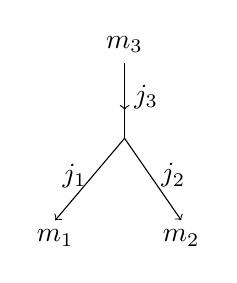
\begin{tikzpicture}[baseline=(current bounding box.center),x=0.8cm,y=0.8cm]
\draw (0,1.2)--(0,0);
\draw[->] (0,0.95)--(0,0.45);
\draw[->] (0,0)--(-1.1,-1.3);
\draw[->] (0,0)--(0.9,-1.3);
\node[above] at (0,1.2) {$m_3$};
\node[right] at (0,0.65) {$j_3$};
\node[left] at (-0.45,-0.60) {$j_1$};
\node[right] at (0.43,-0.59) {$j_2$};
\node[below] at (-1.1,-1.3) {$m_1$};
\node[below] at (0.9,-1.3) {$m_2$};
\end{tikzpicture}
\tag{22}
\end{equation*}

\EnglishSourceFrame{GELFAND-P001466}{unlabelled}
\begin{equation*}
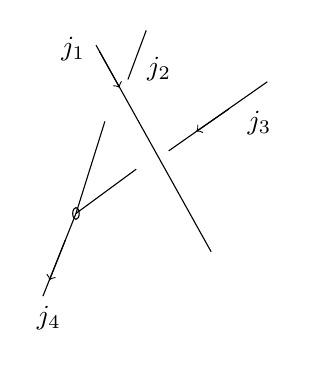
\begin{tikzpicture}[baseline=(current bounding box.center),x=0.75cm,y=0.75cm]
\draw (-0.5,2.6)--(1.45,-0.9);
\draw[->] (-0.44,2.49)--(-0.10,1.88);
\draw (0.35,2.85)--(0.04,2.02);
\draw (-0.35,1.31)--(-0.84,-0.25)--(-1.4,-1.65);
\draw[->] (-1.02,-0.70)--(-1.29,-1.38);
\draw (2.40,1.98)--(0.73,0.81);
\draw[->] (1.75,1.52)--(1.20,1.14);
\draw (0.18,0.50)--(-0.84,-0.25);
\draw (-0.84,-0.25) ellipse (0.055 and 0.10);
\node[left] at (-0.52,2.54) {$j_1$};
\node[right] at (0.20,2.20) {$j_2$};
\node[right] at (1.90,1.28) {$j_3$};
\node[below] at (-1.30,-1.66) {$j_4$};
\end{tikzpicture}
\quad =\quad
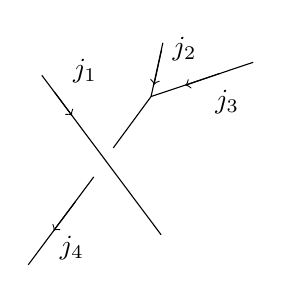
\begin{tikzpicture}[baseline=(current bounding box.center),x=0.75cm,y=0.75cm]
\draw (-1.4,1.8)--(0.62,-0.9);
\draw[->] (-1.18,1.51)--(-0.89,1.12);
\draw (0.65,2.35)--(0.45,1.44);
\draw[->] (0.63,2.24)--(0.50,1.64);
\draw (2.18,2.02)--(0.45,1.44)--(-0.19,0.57);
\draw[->] (1.61,1.83)--(1.03,1.63);
\draw (-0.52,0.08)--(-1.63,-1.41);
\draw[->] (-0.83,-0.34)--(-1.20,-0.83);
\node[above] at (-0.67,1.50) {$j_1$};
\node[right] at (0.65,2.25) {$j_2$};
\node[below] at (1.74,1.71) {$j_3$};
\node[right] at (-1.26,-1.13) {$j_4$};
\end{tikzpicture}
\tag{23}
\end{equation*}

\begin{equation*}
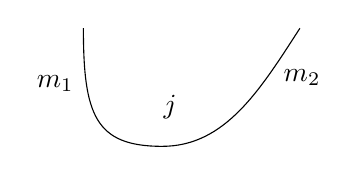
\begin{tikzpicture}[baseline=(current bounding box.center),x=1cm,y=1cm]
\draw (-1.2,0.8).. controls (-1.2,-0.3) and (-1.05,-0.7)..(-0.2,-0.7)
 .. controls (0.6,-0.7) and (1.04,0.01)..(1.55,0.8);
\node[left] at (-1.2,0.1) {$m_1$};
\node[right] at (1.22,0.17) {$m_2$};
\node at (-0.10,-0.20) {$j$};
\end{tikzpicture}
\longrightarrow (-1)^{m_1}q^{m_1}\delta_{m_1,-m_2}
\tag{24}
\end{equation*}
$-j\le m_i\le j,\quad i=1,2.$

(25)
\begin{center}
\begin{tikzpicture}[baseline=(current bounding box.center),x=1cm,y=1cm]
\draw[->] (0.9,-0.1).. controls (0.7,1.2) and (-0.1,0.7)..(-0.9,-0.1);
\node[below] at (-0.9,-0.1) {$m_1$};
\node[below] at (0.9,-0.1) {$m_2$};
\end{tikzpicture}
$\longrightarrow$
\EnglishUnclear{GELFAND-P001466}{eq25-cancelled-exponent}{$(-1)^{m_1}q^{-m_1/2}\delta_{m_1,-m_2}$}
\end{center}
[In the exponent of $(-1)$, to the right of $m$, is a densely crossed-out sign.]

The following equalities hold:

(26) \EnglishSourceFigure{GELFAND-P001466}{eq26-vertex-arrow}{An equality of two trivalent drawings. On the left, $j_1$ enters the vertex from upper left, with an arrow down and right; $j_2$ rises on the right, bends left in an arc and reaches the vertex, with upward arrows on the right-hand portion and a leftward arrow on the arc; $j_3$ leaves the vertex downwards, with a downward arrow. On the right, $j_1$ enters the vertex from above; $j_3$ leaves it down and left, with an arrow away from the vertex. The $j_2$ branch runs geometrically down and right, but its arrow is heavily retraced. Protruding visible strokes permit an arrow toward the vertex, up and left; the final direction is not established from the original.}

\par\medskip\noindent
\begin{minipage}[c]{0.48\linewidth}\centering
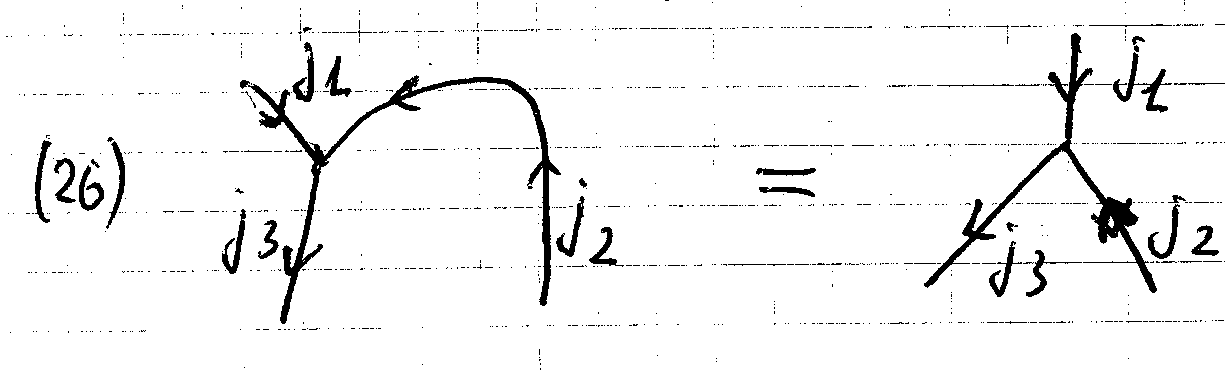
\includegraphics[width=\linewidth]{figures/gelfand-p001466-eq26-vertex-arrow-original.png}
\par\smallskip{\footnotesize Original manuscript diagram: GELFAND-P001466\par}
\end{minipage}\hfill
\begin{minipage}[c]{0.48\linewidth}\centering
\resizebox{\linewidth}{!}{% Partial recreation: no direction is chosen on the retraced right j_2 branch.
\begin{tikzpicture}[x=0.012cm,y=-0.012cm,line width=0.6pt]
\path[use as bounding box] (0,0) rectangle (1225,370);
\draw (245,84)--(318,165)--(290,324);
\draw[->] (260,100)--(288,132);\draw[->] (309,215)--(298,284);
\draw (318,165)..controls(410,72)and(510,33)..(535,104)..controls(551,171)and(550,250)..(548,331);
\draw[->] (550,245)--(549,156);\draw[->] (465,80)--(401,96);
\node at (319,76) {$j_1$};\node at (585,245) {$j_2$};\node at (256,249) {$j_3$};
\node at (790,180) {$=$};
\draw (1075,38)--(1067,144)--(925,315);\draw (1067,144)--(1153,290);
\draw[->] (1073,49)--(1069,104);\draw[->] (1010,212)--(965,263);
\draw[line width=1.4pt] (1100,201)--(1121,237);
\draw (1101,216)--(1114,202);\draw (1107,226)--(1127,217);
\node at (1145,74) {$j_1$};\node at (1015,300) {$j_3$};\node at (1200,251) {$j_2$};
\end{tikzpicture}
}
\par\smallskip{\footnotesize Partial recreation of visible strokes; uncertain labels and connections remain explicit.\par}
\end{minipage}\par\medskip


\begin{equation*}
\begin{tikzpicture}[baseline=(current bounding box.center),x=0.9cm,y=0.9cm]
\draw (-0.4,1.65).. controls (0.05,0.8) and (0.4,-0.7)..(1.15,-0.8)
 .. controls (2.9,-1.0) and (2.7,2.45)..(1.05,1.3)--(0.40,0.85);
\draw[->] (-0.32,1.49)--(-0.09,1.04);
\draw[->] (0.80,-0.69)--(1.24,-0.83);
\draw[->] (1.29,1.44)--(0.91,1.20);
\draw (-0.02,0.45).. controls (-0.58,0.06) and (-0.91,-0.50)..(-1.50,-0.90);
\draw[->] (-0.52,-0.01)--(-0.96,-0.48);
\node[left] at (-0.66,0.30) {$j$};
\end{tikzpicture}
=(-1)^j q^{\frac{j(j+1)}{2}}\quad
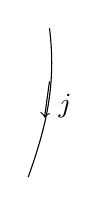
\begin{tikzpicture}[baseline=(current bounding box.center),x=0.9cm,y=0.9cm]
\draw (0.05,1.1).. controls (0.15,0.3) and (0,-0.3)..(-0.25,-1.0);
\draw[->] (0.05,0.35)--(-0.02,-0.16);
\node[right] at (0.04,0) {$j$};
\end{tikzpicture}
\tag{27}
\end{equation*}

(28)
\begin{center}
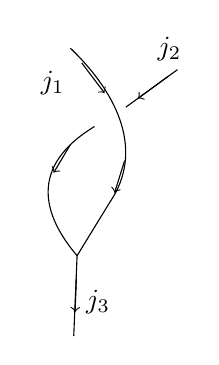
\begin{tikzpicture}[baseline=(current bounding box.center),x=0.85cm,y=0.85cm]
\draw (-0.45,2.2).. controls (0.28,1.5) and (0.65,0.65)..(0.14,-0.10)
 --(-0.35,-0.9)--(-0.40,-2.1);
\draw[->] (-0.28,1.98)--(0.06,1.53);
\draw[->] (0.36,0.52)--(0.21,0.04);
\draw[->] (-0.36,-1.23)--(-0.38,-1.74);
\draw (1.15,1.88)--(0.38,1.32);
\draw[->] (1.01,1.78)--(0.56,1.45);
\draw (-0.09,1.03).. controls (-1.08,0.43) and (-0.86,-0.30)..(-0.35,-0.9);
\draw[->] (-0.45,0.76)--(-0.70,0.34);
\node[left] at (-0.39,1.68) {$j_1$};
\node[above] at (1.03,1.87) {$j_2$};
\node[right] at (-0.36,-1.59) {$j_3$};
\end{tikzpicture}
$=$
\EnglishUnclear{GELFAND-P001466}{eq28-coefficient-j}{$(-1)^{j_1+j_2-j}q^{\frac{j(j+1)-j_1(j_1+1)-j_2(j_2+1)}{4}}$}
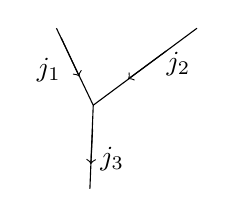
\begin{tikzpicture}[baseline=(current bounding box.center),x=0.85cm,y=0.85cm]
\draw (-0.55,1.15)--(0,0)--(-0.05,-1.25);
\draw (1.55,1.15)--(0,0);
\draw[->] (-0.48,1.01)--(-0.21,0.43);
\draw[->] (1.09,0.81)--(0.52,0.39);
\draw[->] (-0.01,-0.36)--(-0.035,-0.88);
\node[left] at (-0.34,0.53) {$j_1$};
\node[right] at (0.95,0.62) {$j_2$};
\node[right] at (-0.04,-0.80) {$j_3$};
\end{tikzpicture}
\end{center}

This makes it possible to construct invariants of links, braids
and knotted ribbons.

\EnglishSourceFrame{GELFAND-P001467}{66}
\underline{Link invariants.}

Fix an orientation and a direction $t$.

(29)
\EnglishSourceFigure{GELFAND-P001467}{x58-y247-x646-y638}{On the left is a vertical upward arrow labelled $t$. On the right is a curved loop: the upper and lower bends and two places in the upper middle portion are circled with ovals. Above the left middle place is $m_i$; to the right of the loop is $j$. Arrows are visible on the curve; the middle lines cross, and there are gaps on the right. The exact passage of the branches and all arrows beneath overlapping strokes is not established.}

\par\medskip\noindent
\begin{minipage}[c]{0.48\linewidth}\centering
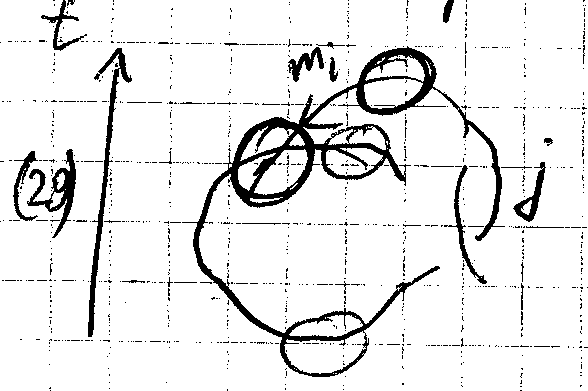
\includegraphics[width=\linewidth]{figures/gelfand-p001467-x58-y247-x646-y638-original.png}
\par\smallskip{\footnotesize Original manuscript diagram: GELFAND-P001467\par}
\end{minipage}\hfill
\begin{minipage}[c]{0.48\linewidth}\centering
\resizebox{\linewidth}{!}{% Partial trace only. Gaps and crossed strokes do not certify the knot topology.
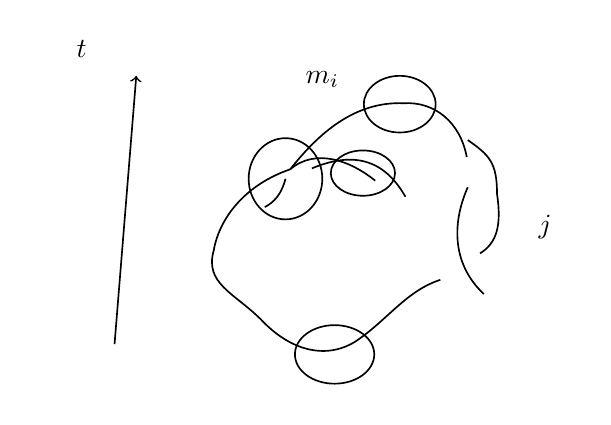
\begin{tikzpicture}[x=0.012cm,y=-0.012cm,line width=0.6pt]
\path[use as bounding box] (0,0) rectangle (588,391);
\draw[->] (92,335)--(115,51);\node at (57,23) {$t$};
\draw (278,150)..controls(231,166)and(203,201)..(197,236)
 ..controls(187,271)and(219,281)..(247,309)
 ..controls(277,341)and(314,352)..(346,333)
 ..controls(380,311)and(400,279)..(437,267);
\draw (278,150)..controls(308,112)and(346,78)..(398,80)
 ..controls(431,78)and(458,100)..(465,137);
\draw (466,119)..controls(489,135)and(497,143)..(497,176)
 ..controls(502,209)and(497,228)..(479,239);
\draw (466,169)..controls(448,210)and(451,252)..(483,282);
\draw (278,150)..controls(305,127)and(342,141)..(368,162);
\draw (301,149)..controls(337,134)and(374,133)..(400,179);
\draw (273,160)..controls(269,176)and(261,185)..(251,190);
\draw (394,81) ellipse[x radius=38,y radius=30];
\draw (273,160) ellipse[x radius=39,y radius=43];
\draw (355,154) ellipse[x radius=34,y radius=24];
\draw (325,346) ellipse[x radius=42,y radius=31];
\node at (312,55) {$m_i$};\node at (548,211) {$j$};
\end{tikzpicture}
}
\par\smallskip{\footnotesize Partial recreation of visible strokes; uncertain labels and connections remain explicit.\par}
\end{minipage}\par\medskip


\underline{Elementary fragments:}

1) fixed points where the normal is $\parallel$ to the $t$ axis (the chosen direction)

2) crossing points

Place numbers $m_i$ at the joins of elementary fragments so that
\begin{equation*}
-j\leq m_i\leq j \qquad (j\ \text{chosen arbitrarily})
\end{equation*}

\begin{equation*}
\sum_{\{m\}}\prod_{\substack{\text{over all}\\\text{elementary}\\\text{fragments}}}
v(\{m\})=\varphi_{j_1\ldots j_k}(D_L,q)
\tag{30}
\end{equation*}
\EnglishUnclear{GELFAND-P001467}{x656-y1355-x935-y1489}{In (30), the letter before $(\{m\})$ is $v$ or $\nu$.}

\textit{[A pointer leads from this letter to the caption:]} matrix elements calculated above

(31) \underline{Theorem}
\begin{equation*}
I_{j_1\ldots j_k}(L,q)
=q^{\sum_i N_+^i(D_L)-N_-^i(D_L)}\varphi_{\{j\}}(D_L,q)
\end{equation*}
\EnglishUnclear{GELFAND-P001467}{x1935-y1670-x2000-y1726}{[After $N_-^i(D_L)$ in the exponent, a small superscript sign is crossed out; its reading is not established.]}

--- a link invariant (independent of the projection of the knot onto the plane)

$N_\pm^i$ is the number of times the $i$th strand passes \underline{under} and \underline{over}.

This includes the Jones invariant.

One can \EnglishUnclear{GELFAND-P001467}{x520-y2610-x734-y2730}{[An illegible crossed-out word]} construct knot invariants for $\forall$ simple Lie algebra.

There is a conjecture that the $SL_2$ invariants suffice.

There are also $6j$ symbols.

\EnglishSourceFrame{GELFAND-P001468}{unlabelled}
\underline{25.4.88.}\quad\underline{Gelfand's seminar}
\qquad
\underline{Ushveridze}
\EnglishUnclear{GELFAND-P001468}{x1260-y33-x1400-y148}{[Illegible crossed-out signs]}
\underline{Alexander Grigorievich.}
\EnglishUnclear{GELFAND-P001468}{x2040-y40-x2310-y150}{[An illegible crossed-out entry]}

\underline{The Riccati equation and quasi-exactly solvable problems.}

\begin{equation*}
y'(\lambda)+y^2(\lambda)+2B(\lambda)y(\lambda)+C(\lambda)=0,
\tag{1}
\end{equation*}
\begin{equation*}
B(\lambda)=\sum_{\alpha=1}^N b_\alpha\Delta(\lambda-a_\alpha),
\tag{2}
\end{equation*}
\begin{equation*}
C(\lambda)=\sum_{\alpha=1}^N c_\alpha\Delta(\lambda-a_\alpha).
\tag{3}
\end{equation*}

Seek a solution of (1) in the form
\begin{equation*}
y(\lambda)=\sum_{i=1}^M\Delta(\lambda-\lambda_i)
\tag{4}
\end{equation*}

Then, for certain
\textit{[insertion above the line:]} conditions on $\Delta$
\EnglishUnclear{GELFAND-P001468}{x1000-y1240-x1248-y1328}{finding [source abbreviation]}
\textit{[end of insertion]}
parameter values, this reduces to algebraic equations:
\begin{equation*}
\left\{
\begin{aligned}
&\sum_{i=1}^{M}{}'\Delta(\lambda_i-\lambda_k)
 +\sum_{\alpha=1}^{N}b_\alpha(\lambda_i-a_\alpha)=0\\
&\text{(sum over }i\neq k\text{)}\\
&c_\alpha=2b_\alpha\sum_{i=1}^{M}\Delta(\lambda_i-a_\alpha)
\end{aligned}
\right.
\tag{5}
\end{equation*}
\EnglishUnclear{GELFAND-P001468}{x350-y1390-x1615-y1675}{[In the first line of (5), $b_\alpha$ is followed directly by $(\lambda_i-a_\alpha)$; the first summation has $i=1$, and the argument of $\Delta$ is $\lambda_i-\lambda_k$. As in the source.]}

(6) \underline{Properties of $\Delta$ and $\Omega$}
\qquad (a generalization of addition theorems for elliptic functions)

\begin{equation*}
\begin{aligned}
1)\quad &\Delta(\lambda_1)\Delta(\lambda_2)+\Delta(\lambda_2)\Delta(\lambda_3)
+\Delta(\lambda_3)\Delta(\lambda_1)\\
&\qquad +\Omega(\lambda_1)+\Omega(\lambda_2)+\Omega(\lambda_3)=0\\
&\text{when }\lambda_1+\lambda_2+\lambda_3=0
\end{aligned}
\end{equation*}
\begin{equation*}
2)\quad \Delta(\lambda)+\Delta(-\lambda)=0
\end{equation*}

3) \EnglishUnclear{GELFAND-P001468}{x435-y2450-x570-y2578}{[A crossed-out formula; a sign resembling $\Delta$ is distinguishable, the rest is not established]}
$\Omega(\lambda)-\Omega(-\lambda)=0$

(7) \underline{Examples of solutions of system (6)}

\begin{equation*}
1)\quad \Delta(\lambda)=\frac{1}{\lambda},\qquad \Omega(\lambda)=0;
\end{equation*}
\EnglishUnclear{GELFAND-P001468}{x1335-y2810-x1494-y2960}{[Signs to the right of the first pair of formulas are crossed out; a triangular sign resembling $\Delta$ is distinguishable.]}

\begin{equation*}
2)\quad \Delta(\lambda)=\omega\operatorname{ctg}\omega\lambda,
\qquad \Omega(\lambda)=\frac{\omega^2}{3}
\end{equation*}
\begin{equation*}
3)\quad \Delta(\lambda)=\zeta(\lambda),
\qquad \Omega(\lambda)=\zeta^2(\lambda)-\wp(\lambda)
\end{equation*}
\textit{[Below $\zeta(\lambda)$, with a short pointer:]} Weierstrass function
\qquad (quasiperio

\EnglishSourceFrame{GELFAND-P001469}{67}
\underline{Applications.}

A. $y=\dfrac{f'}{f}\quad\Rightarrow$ the Schrodinger equation for $f$;

A solution of (6) with a singularity at $0$ satisfies the equation
\begin{equation*}
\Delta'(\lambda)+\Delta^2(\lambda)=2\Omega(\lambda)+\Omega(0)
\tag{8}
\end{equation*}

\begin{center}
\begin{tikzpicture}
\node[draw,inner sep=8pt] (cancelled) at (0,0) {$\begin{aligned}
\Omega(\lambda)&=\frac{\omega^2}{3}\\
\Omega(\lambda)&=\zeta^2(\lambda)-\wp(\lambda)
\end{aligned}$};
\draw (cancelled.north west) -- (cancelled.south east);
\draw (cancelled.south west) -- (cancelled.north east);
\end{tikzpicture}
\end{center}

(9) $\Delta_0(b\lambda)+a\lambda$ is the general solution of system (6), where

$\Delta_0$ is one of the functions in example (6).
\EnglishUnclear{GELFAND-P001469}{x438-y860-x2110-y1115}{[In (9) there is no external multiplier before $\Delta_0(b\lambda)$; the next line says “example (6)”. As in the source.]}

B. This also gives Bethe-ansatz solutions for spin systems.

C. $(5)\Leftrightarrow$
\textit{[insertion above the line:]} in the case
\EnglishUnclear{GELFAND-P001469}{x825-y1238-x1030-y1340}{[An illegible crossed-out entry before $(7)_1$]}
$(7)_1$ \textit{[end of insertion]}
the equilibrium condition for a classical system of charged particles, of
\underline{two types:} stationary particles with coordinates $a_\alpha$ and charges $b_\alpha$;
mobile particles with
\EnglishUnclear{GELFAND-P001469}{x800-y1425-x1005-y1558}{[An illegible crossed-out word; “coord.” is inserted above it]}
$\lambda_i$ and charge $1$.

\textit{[On the right:]} \underline{Potential:}
$q_iq_k\ln|\lambda_i-\lambda_k|$

In case $(7)_2$,
particles on a circle with potential
\begin{equation*}
q_iq_k\ln|\sin(\lambda_i-\lambda_k)|
\end{equation*}

In case $(7)_3$, the interaction potential is
\begin{equation*}
q_iq_k\ln\theta(\lambda_i-\lambda_k)
\end{equation*}

(10) \underline{For the Schrodinger equation}

$\lambda_i$ are the nodes of the wave function.

In the Coulomb system

\EnglishUnclear{GELFAND-P001469}{x500-y2640-x570-y2745}{[A sign before $\lambda_i$ is crossed out; its reading is not established]}
$\lambda_i$ are the coordinates of charged particles.

In the Bethe equation, $\lambda_i$ are rapidities.

\begin{center}
\rule{2cm}{0.4pt}\quad$\cdot$\quad\rule{2cm}{0.4pt}
\end{center}

Stability of the quantum-mechanical system $\Leftrightarrow$ stability of the Coulomb system

\begin{center}
\rule{2cm}{0.4pt}\quad$\cdot$\quad\rule{2cm}{0.4pt}
\end{center}

\underline{What should one do with partial integrability?}
(with an incomplete system of integrals)

\begin{equation*}
H=H_0+L_1(H_1-c_1)+L_2(H_2-c_2),
\qquad L_j\text{ --- operators}
\tag{11}
\end{equation*}
Let $H_j$ commute, $j=0,1,2$.

\EnglishSourceFrame{GELFAND-P001470}{unlabelled}
\EnglishUnclear{GELFAND-P001470}{top-left-label}{[A crossed-out note in the left margin; illegible]}

Consider a common eigenvector of $H_0,H_1,H_2$; then
\EnglishUnclear{GELFAND-P001470}{top-line-cancellation}{[Crossed out; illegible]}

If $c_j$ are the eigenvalues of $H_j$, they determine an eigenvalue of
\EnglishUnclear{GELFAND-P001470}{top-right-cancellation}{[Crossed out; illegible]} $H$
(and we \EnglishUnclear{GELFAND-P001470}{top-eigenvectors-verb}{know} the eigenvectors---\underline{as many as} the degeneracy multiplicity).

In this language
\begin{equation*}
\begin{aligned}
\text{quantum nonlinear Schrodinger}&\ \Longleftrightarrow\ \text{harmonic oscillator}\\
\text{[crossed out: oper.] energy}&\ \Longleftrightarrow\ \text{particle-number operator}
\end{aligned}
\end{equation*}

\begin{center}— . —\end{center}

The spectrum of $H_i$ is found from the Bethe-ansatz equations.

\begin{center}— . —\end{center}

\underline{Reference:}

Brief Reports on Physics of FIAN.

\underline{Passing from the Riccati equation to the Schrodinger equation}

This can be done in innumerable ways.
\begin{equation*}
y=\frac{f'}{f}\quad\Longrightarrow
\end{equation*}
\begin{equation*}
f''+2Bf'+Cf=0
\qquad\text{(the independent variable here is $\lambda$)}
\tag{12}
\end{equation*}

Multiply [inserted above the line: (12)] by an arbitrary function $A$ and then eliminate $f'$.
$\Longrightarrow$ [below the line: (by changing the independent variable!)]
$\Longrightarrow$ one obtains the Schrodinger equation
\begin{equation*}
\left[-\frac{\partial^2}{\partial x^2}+V(x)\right]\Psi(x)=0
\tag{13}
\end{equation*}

Each $A$ gives its own potential $V$.

The function $A$ can be chosen so that information about the numbers
\EnglishUnclear{GELFAND-P001470}{lower-number-cancellation}{[Crossed out; illegible]}
$c_\alpha,\lambda_i$ is concentrated in the part of the potential independent of $x$:
\begin{equation*}
V(x)=U(x)-E(\lambda_i)
\tag{14}
\end{equation*}

Then (13) \EnglishUnclear{GELFAND-P001470}{lower-equation-cancellation}{[Crossed out; illegible]}
$\sim$ the Schrodinger equation.

For this one needs
\begin{equation*}
A(\lambda)=\prod_{\alpha=1}^{N}\Xi(\lambda-a_\alpha),
\qquad\frac{\Xi'(\lambda)}{\Xi(\lambda)}=\Delta(\lambda)
\tag{15}
\end{equation*}

Passing to $x$:
\begin{equation*}
x=\int^{\lambda(x)}\frac{d\lambda}{\sqrt{A(\lambda)}}
\tag{16}
\end{equation*}

\EnglishSourceFrame{GELFAND-P001471}{68}
(17) \EnglishUnclear{GELFAND-P001471}{top-initial-cancellation}{[Crossed out; illegible]}
In case $(7)_1$:
\begin{equation*}
A(\lambda)=\prod_{\alpha=1}^{N}(\lambda-a_\alpha)
\end{equation*}
\EnglishUnclear{GELFAND-P001471}{top-line-cancellation}{[Crossed out: a linear function of $\lambda$]}

($\Xi$ is a linear function of $\lambda$.)

This gives the Jacobi transformation (16).

\underline{Use the Coulomb analogy to classify}
exactly and quasi-exactly solvable problems.

Let $N=2$ in (2)–(3).

\begin{center}
\begin{tikzpicture}[x=1cm,y=1cm]
\draw (0,0) -- (5.2,0);
\draw (1.2,-0.10) -- (1.2,0.10);
\draw (3.2,-0.10) -- (3.2,0.10);
\node[above] at (1.2,0.20) {$b_1$};
\node[above] at (3.2,0.20) {$b_2$};
\node[below] at (1.2,-0.15) {$a_1$};
\node[below] at (3.2,-0.15) {$a_2$};
\node[right] at (5.35,-0.28) {$\lambda$};
\end{tikzpicture}
\end{center}

$a_1,a_2$ are the coordinates of the stationary particles (classical).

The mobile particles $\underset{\text{coord.}}{\{\lambda_i\}}$ number $M$.

(18) \EnglishUnclear{GELFAND-P001471}{middle-potential-cancellation}{[Crossed out; illegible]}
The potential $V$ does not contain $M$ (!) $\Longrightarrow$ we have an exactly solvable model.

(19) Let $b_1,b_2>0$.

\begin{center}
\begin{tikzpicture}[x=1cm,y=1cm]
\draw (0,0) -- (4.2,0);
\draw (0,-0.16) -- (0,0.18);
\draw (4.06,-0.18) -- (4.22,0.19);
\node[above] at (0,0.22) {$b_1$};
\node[above] at (4.2,0.22) {$b_2$};
\draw (1.08,-0.12) -- (1.10,0.17);
\draw (1.62,-0.13) -- (1.68,0.16);
\draw (2.12,-0.13) -- (2.20,0.12);
\draw (2.47,-0.13) -- (2.56,0.12);
\draw (2.85,-0.13) -- (2.95,0.10);
\draw (3.25,-0.15) -- (3.37,0.17);
\end{tikzpicture}
\end{center}

The particles inside will not escape because of repulsion.
$\Longrightarrow\ \exists\min\ \Longrightarrow\ \exists$ a solution of the Schrodinger equation
with $M$ nodes $\Longrightarrow$ integrability!!!

(all wave functions are found!!)

Another case

(20)
\begin{center}
\par\medskip\noindent
\begin{minipage}[c]{0.48\linewidth}\centering
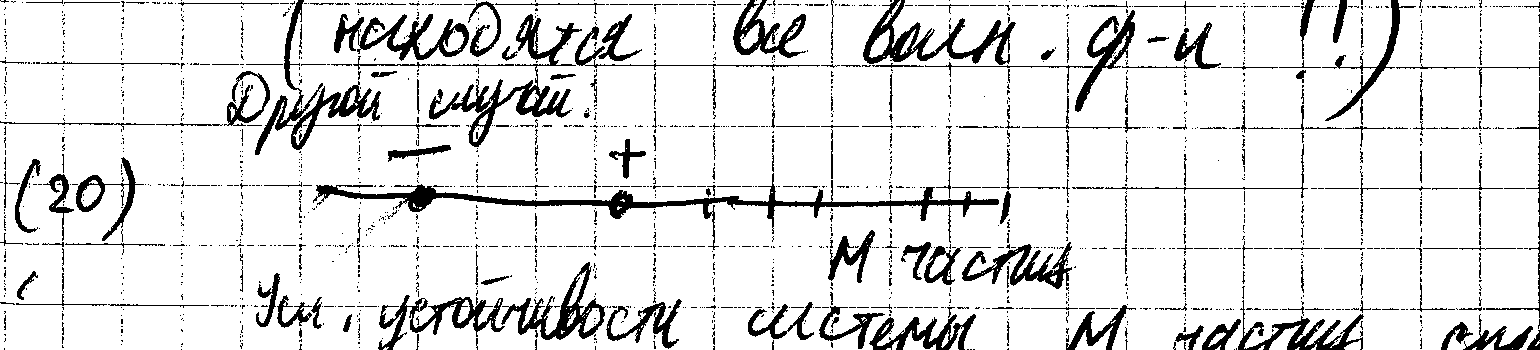
\includegraphics[width=\linewidth]{figures/gelfand-p001471-diagram20-full-original-r2.png}
\par\smallskip{\footnotesize Original manuscript diagram: GELFAND-P001471\par}
\end{minipage}\hfill
\begin{minipage}[c]{0.48\linewidth}\centering
\resizebox{\linewidth}{!}{\begin{tikzpicture}[x=1cm,y=1cm]
\draw (0,0) -- (7.0,0);
\fill (1.0,0) circle (0.075);
\draw (3.0,0) circle (0.065);
\node[above] at (1.0,0.20) {$-$};
\node[above] at (3.0,0.20) {$+$};
\draw (3.92,-0.14) -- (3.94,0.10);
\draw[<-] (4.12,0) -- (4.32,0);
\draw (4.55,-0.15) -- (4.55,0.17);
\draw (5.00,-0.13) -- (5.08,0.13);
\draw (6.10,-0.14) -- (6.18,0.18);
\draw (6.52,-0.11) -- (6.54,0.10);
\draw (7.06,-0.16) -- (7.14,0.14);
\node[below] at (5.85,-0.24) {$M$ particles};
\end{tikzpicture}
}
\par\smallskip{\footnotesize Existing native recreation; unclear left strokes are described in the reading note.\par}
\end{minipage}\par\medskip

\end{center}
\EnglishSourceFigure{GELFAND-P001471}{diagram20-faint-strokes}{In diagram (20), the left end of the horizontal line is thickened and has sloping strokes; an arrowhead cannot be reliably distinguished. Below this end and below the dark point on the left, faint strokes descend to the left; their exact purpose and connection with the thick strokes are unclear.}
\EnglishUnclear{GELFAND-P001471}{margin-below20}{[In the left margin below (20): a short separate sloping stroke]}

Stability condition for the system of $M$ particles to the right of $b_2$:
\begin{equation*}
\underline{b_1+b_2+M<0}
\tag{21}
\end{equation*}

(they do not approach $b_2$, but do not escape to $\infty$ either)

But this condition fails for large $M$!
$\Longrightarrow$ only finitely many levels occur.

\EnglishSourceFrame{GELFAND-P001472}{unlabelled}
Choosing different intervals gives different problems.

This yields exactly solvable models (magnetic systems).

\underline{\underline{A. Beilinson}}

\underline{on work by \EnglishUnclear{GELFAND-P001472}{upper-atiya-name}{Ati [source name]}}

\underline{New invariants of 3- and 4-dimensional manifolds}

(semi-infinite Morse theory)

\begin{equation*}
\underset{\substack{\text{natural}\\\infty\text{-dimensional manifold}}}{X}
\overset{f}{\longrightarrow}\mathbb{R}
\qquad\text{--- a Morse function}
\end{equation*}

The critical points contain an $\infty$ number of $+$ and $-$ squares,
but at different points the difference is finite.

New homology groups arise.

Equip the manifold $X$ with a Riemannian metric.

First let $\dim X<\infty$ and let $X$ be compact.

$g$ is the metric,
\begin{equation*}
\tau=\operatorname{grad}f
\end{equation*}

Consider \EnglishUnclear{GELFAND-P001472}{middle-flow-cancellation}{[Crossed out; illegible]}
[inserted above the line: trajectories] of the field $\tau$.

They are of two types: points [below the line: (critical)] and trajectories joining 2 critical points.

If the metric is in general position, consider the space $T(x_1,x_2)$
of all trajectories going from $x_1$ to $x_2$. Then
\begin{equation*}
\dim T(x_1,x_2)=\operatorname{ind}_{x_1}f-\operatorname{ind}_{x_2}f-1
\tag{1}
\end{equation*}

In particular, \underline{if the indices differ by 1, this is a discrete set.}

Let
\begin{equation*}
\operatorname{ind}_{x_1}f=\operatorname{ind}_{x_2}f+1
\tag{2}
\end{equation*}

Then each $\forall$ trajectory joining $x_1$ and $x_2$ is assigned a number $\pm1$,
depending on the given orientations.
\EnglishUnclear{GELFAND-P001472}{bottom-orientation-cancellation}{[Crossed out; illegible]}
[inserted above the line: $T(x_1,x_2)$] Now construct a complex.

\EnglishSourceFrame{GELFAND-P001473}{69}
\begin{equation*}
\longrightarrow C_i\overset{d}{\longrightarrow}C_{i-1}\longrightarrow\ldots
\tag{3}
\end{equation*}

$C_i$ is the vector space with basis $\{x_\alpha\}$, $\operatorname{ind}x_\alpha=i$.

$d$ is specified by a matrix;

an entry is indexed by a pair of points of adjacent index, $x_1,x_2$.
\begin{equation*}
d=\Vert d_{x_1x_2}\Vert,
\end{equation*}
\begin{equation*}
d_{x_1x_2}=\sum_{\substack{\text{trajectories}\\\text{joining }x_1,x_2}}\pm1
\tag{4}
\end{equation*}

\begin{center}
\rule{12mm}{0.4pt}\quad$\cdot$\quad\rule{12mm}{0.4pt}
\end{center}

Let $M$ be a compact 3-dimensional manifold.

Consider the space of all [inserted above the line: irreducible] connections $C$
[crossed out: \EnglishUnclear{GELFAND-P001473}{mid-cancelled-after-c}{illegible}].

[Below “connections”: (Hermitian)]

on the trivial 2-dimensional bundle over $M$.

Such a connection has the form $d+A$, where
\begin{equation*}
A\in\Omega^1(M)\otimes\mathrm{su}_2
\end{equation*}

Consider them up to gauge equivalence.
\begin{equation*}
G\text{ --- the gauge group }SU_2^M;\qquad
X=C/G\text{ --- the orbit space}
\end{equation*}
$X$ is the main manifold.

Define a Morse function on $X$, or more precisely its differential:
$\nu$ is a 1-form on $C$.

[“Tangent vector to C” has a wavy underline in the source.]
\underline{A tangent vector to $C$}: a matrix-valued 1-form

($C$ is an affine space)
\begin{equation*}
B\in\Omega^1(M)\otimes\mathrm{su}_2.
\end{equation*}
\begin{equation*}
\langle\nu,B_\nabla\rangle
=\int_M\operatorname{Tr}(F_\nabla\cdot B),
\qquad B\in\Omega^1(M)\otimes\mathrm{su}_2
\tag{5}
\end{equation*}
[Below $F_\nabla$, with a pointer: curvature of $A$]

[On the right:] $F_\nabla\cdot B$ is the exterior product (a 3-form!!).
\begin{equation*}
F_\nabla=dA+\frac{1}{2}[A,A]
\tag{6}
\end{equation*}

\EnglishSourceFrame{GELFAND-P001474}{unlabelled}
[The source heading has a wavy underline.]
(7) \underline{Properties of $\nu$}.

1. $\nu$ is pulled back from $X$.

2. $\nu$ is a closed 1-form.

3. [Insertion above the line before $\nu$: Antiderivative [abbr.]] $\nu$ is a secondary characteristic class for
\EnglishUnclear{GELFAND-P001474}{upper-class-symbol}{$c_2$} (Chern class)

--- the Chern--Simons class for $c_2$:
\begin{equation*}
\int_{M\times[0,1]}\operatorname{Tr}(F_{\widetilde\nabla})^2
\tag{8}
\end{equation*}
where

(9) [Crossed out: \EnglishUnclear{GELFAND-P001474}{mid-cancelled-notation}{$A_\nabla$}]
$\widetilde\nabla$ is a connection on the trivial bundle over $M\times[0,1]$

with potential at the point $(x,t)$ equal to $tA$.

This connection is on $C$, rather than on $X$.

[Small insertion between the lines:]
\underline{Remark by \EnglishUnclear{GELFAND-P001474}{mid-remark-initials}{I. M. G.}}:
All this is contained in the “simple” part of the work by Gabr.--Gelf.--Losik.

Look at the critical points.

[A short line is crossed out:
\EnglishUnclear{GELFAND-P001474}{mid-cancelled-line}{illegible}]

These are connections with curvature 0, i.e. integrable connections, i.e.
representations of $\pi_1(M)$.

[“Hessian” has a wavy underline in the source.]
\underline{Hessian}.
\begin{equation*}
\nabla\in C,\qquad
T_{C,\nabla}=\Omega^1(M)\otimes\mathrm{su}_2
\overset{\text{projection}}{\longrightarrow}T_{X,\overline\nabla}
\tag{10}
\end{equation*}
Introduce

[The formula number is corrected:
(\EnglishUnclear{GELFAND-P001474}{lower-equation-label}{11})]
\begin{center}
\EnglishUnclear{GELFAND-P001474}{lower-m-x-notation}{$\nabla_{ad}:\Omega^0(X)\otimes\mathrm{su}_2
\longrightarrow\Omega^1(X)\otimes\mathrm{su}_2,$}
\end{center}
by the formula
\begin{equation*}
\nabla_{ad}(\varphi)=d\varphi+[A,\varphi]
\tag{12}
\end{equation*}
and then
\begin{equation*}
T_{X,\nabla}=
\frac{\Omega^1(X)\otimes\mathrm{su}_2}
{\nabla_{ad}\bigl(\Omega^0(X)\otimes\mathrm{su}_2\bigr)}
\tag{13}
\end{equation*}
This holds for any connection.

